\documentclass{artisubssubssubssubssubscle}
\usepackage{graphicx}
\usepackage{multirow}
\usepackage{amsmath}

\title{Latex Document}
\author{Milinda Barua}
\date{\today}
\begin{document}

\maketitle

\section{Introduction}
\subsection{fig, table}
\begin{figure}[h]
    \centering
    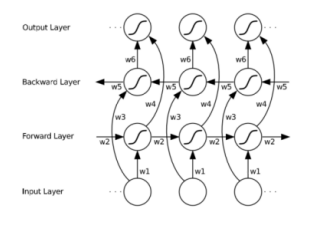
\includegraphics[width=0.6\textwidth]{./assets/image1.png}
    \caption{Graphical representation}
    \label{fig:graphical_representation}
\end{figure}


\begin{table}[h!]
    \centering
    % \begin{tabular}{c|c|c}
\begin{tabular}{ |p{3cm}|p{3cm}|p{3cm}|  }
 \hline
 Country Name or Area Name& ISO ALPHA 2 Code &ISO ALPHA 3 Code\\
 \hline
 Afghanistan & AF & AFG\\
 Aland Islands & AX & ALA\\
 \hline
 Albania & AL & ALB\\
 Algeria & DZ & DZA\\
 American Samoa & AS & ASM\\
 Andorra & AD & AND\\
 Angola & AO & AGO\\
 \hline
    \end{tabular}
    \label{tab:my_label}
\end{table}

\begin{table}[h!]
    \centering
    \begin{tabular}{c c}
        Table: &row table\\
        \hline
        \textbf{first column} & \textbf{second column} \\
        \multirow{2}{*}{\textbf{Multirow}} & X \\
        & X \\
        Cricket & Football \\
        \hline
    \end{tabular}
\end{table}

\subsection{Equation}
\begin{align}
    \text{Precision} &= \frac{TP}{TP + FP} \tag{1}\\
    \text{Recall} &= \frac{TP}{TP + FN} \tag{2}\\
    F1 &= 2 \times \frac{\text{Precision} \times \text{Recall}}{\text{Precision} + \text{Recall}} \tag{3}\\
    \text{Accuracy} &= \frac{TN + TP}{TN + FP + TP + FN} \tag{4}
\end{align}

\subsection{List}
\begin{enumerate}
    \item first item
    \begin{itemize}
        \item apple
        \item mango
    \end{itemize}
    \item second item
    \begin{itemize}
        \item car
        \item bike
    \end{itemize}
\end{enumerate}

\end{document}